%%%%%%%%%%%%%%%%%%%%%%%%%%%%%%%%%%%%%%%
\section{\label{sec:DAGMan}DAGMan Applications}
%%%%%%%%%%%%%%%%%%%%%%%%%%%%%%%%%%%%%%%
\index{DAGMan|(}
\index{directed acyclic graph (DAG)}
\index{Directed Acyclic Graph Manager (DAGMan)}
\index{condor\_submit\_dag}
\index{job!dependencies within}

A directed acyclic graph (DAG) can be used to represent a set of computations
where the input, output, or execution of one or more computations
is dependent on one or more other computations.
The computations are nodes (vertices) in the graph,
and the edges (arcs) identify the dependencies.
Condor finds machines for the execution of programs, but it
does not schedule programs based on dependencies.
The Directed Acyclic Graph Manager (DAGMan) is a meta-scheduler for 
the execution of programs (computations). 
DAGMan submits the programs to Condor in an order represented by
a DAG and processes the results.
A DAG input file describes the DAG, and
further submit description file(s) are used by DAGMan
when submitting programs to run under Condor.

DAGMan is itself executed as a scheduler universe job
within Condor.
As DAGMan submits programs, it monitors log file(s) to 
to enforce the ordering required within the DAG.
DAGMan is also responsible for scheduling, recovery, and reporting
on the set of programs submitted to Condor.

%%%%%%%%%%%%%%%%%%%%%%%%%%%%%%%%%%%%%%%
\subsection{\label{sec:DAGTerminology}DAGMan Terminology}
%%%%%%%%%%%%%%%%%%%%%%%%%%%%%%%%%%%%%%%

To DAGMan, a node in a DAG may encompass more than a single
program submitted to run under Condor.
Figure~\ref{fig:dagman-node} illustrates the elements of a node.

\begin{figure}[hbt]
\centering
\includegraphics{user-man/dagman-node.eps}
\caption{\label{fig:dagman-node}One Node within a DAG}
\end{figure}

At one time,
the number of Condor jobs per node was restricted to one.
This restriction is now relaxed such that all Condor jobs
within a node must share a single cluster number.
See the
\Condor{submit} manual page
for a further definition of a cluster.
A limitation exists such that
all jobs within the single cluster must use the same log file.

As DAGMan schedules and submits jobs within nodes to Condor,
these jobs are defined to succeed or fail based on their
return values.
This success or failure is propagated in well-defined ways to the level of
a node within a DAG.
Further progression of computation
(towards completing the DAG)
may be defined based upon the success or failure of one or more nodes.

The failure of a single job within a cluster
of multiple jobs
(within a single node)
causes the entire cluster of jobs to fail.
Any other jobs within the failed cluster of jobs are
immediately removed.
Each node within a DAG is further defined to succeed or fail,
based upon the return values of a PRE script, the job(s)
within the cluster, and/or a POST script.

%%%%%%%%%%%%%%%%%%%%%%%%%%%%%%%%%%%%%%%
\subsection{Input File Describing the DAG}
%%%%%%%%%%%%%%%%%%%%%%%%%%%%%%%%%%%%%%%

\index{DAGMan!input file example}
The input file used by DAGMan is called a DAG input file.
It may specify eleven types of items:
\begin{enumerate}
\item
A list of the nodes in the DAG which cause the submission of
one or more Condor jobs. Each entry serves to name a node
and specify a Condor submit description file.
\item
A list of the nodes in the DAG which cause the submission of
a data placement job.
Each entry serves to name a node and 
specify the Stork submit description file.
\item
Any processing required to take place before submission of
a node's Condor or Stork job, or after a node's Condor or Stork
job has completed execution.
\item
A description of the dependencies within the DAG.
\item
The number of times to retry a node's execution,
if a node within the DAG fails.
\item
Any definition of macros associated with a node.
\item
A specification of the priority of a node.
\item
A specification of the category of a node.
\item
A maxjobs specification for a given node category.
\item
A node's exit value that causes the entire DAG to abort.
\item
A configuration file.
\end{enumerate}

All items are optional, but there must be at least one \Arg{JOB}
or \Arg{DATA} item.

Comments may be placed in the DAG input file.
The pound character (\verb@#@) as the first character on a
line identifies the line as a comment.
Comments do not span lines.

A simple diamond-shaped DAG, as shown in
Figure~\ref{fig:dagman-diamond}
is presented as a starting point for examples.
This DAG contains 4 nodes.

\begin{figure}[hbt]
\centering
\includegraphics{user-man/dagman-diamond.eps}
\caption{\label{fig:dagman-diamond}Diamond DAG}
\end{figure}


A very simple DAG input file for this diamond-shaped DAG is

\footnotesize
\begin{verbatim}
    # Filename: diamond.dag
    #
    JOB  A  A.condor 
    JOB  B  B.condor 
    JOB  C  C.condor	
    JOB  D  D.condor
    PARENT A CHILD B C
    PARENT B C CHILD D
\end{verbatim}
\normalsize

Each DAG input file key word is described below.

%%%%%%%%%%%%%%%%%%%%%%%%%%%%%%%%%%%%%%%
\subsubsection{\label{dagman:JOB}JOB}

The \Arg{JOB} key word specifies a job to be managed by Condor.
The syntax used for each \Arg{JOB} entry is

\Opt{JOB} \Arg{JobName} \Arg{SubmitDescriptionFileName}
\oOptArg{DIR}{directory} \oOpt{DONE}

A \Arg{JOB} entry maps a \Arg{JobName} to a Condor submit description file.
The \Arg{JobName} uniquely identifies nodes within the
DAGMan input file and in output messages.
Note that the name for each node within the DAG
must be unique.

The key words \Arg{JOB} and \Arg{DONE}
are not case sensitive.
Therefore, \Arg{DONE}, \Arg{Done}, and \Arg{done} are all equivalent.
The values defined for \Arg{JobName} and \Arg{SubmitDescriptionFileName}
are case sensitive, as file names in
the Unix file system are case sensitive.
The \Arg{JobName} can be any string that contains no white space, except
for the strings \Arg{PARENT} and \Arg{CHILD} (in upper, lower, or mixed
case).

The \Arg{DIR} option specifies a working directory
for this node,
from which the Condor job will be submitted,
and from which a \Arg{PRE} and/or
\Arg{POST} script will be run.
Note that a DAG containing \Arg{DIR} specifications cannot
be run in conjunction with the \Arg{-usedagdir} command-line
argument to \Condor{submit\_dag}.  A rescue DAG generated by
a DAG run with the \Arg{-usedagdir} argument will contain
DIR specifications, so the rescue DAG must be run \emph{without}
the \Arg{-usedagdir} argument.

The optional \Arg{DONE} identifies a job as being already
completed.
This is useful in situations where the user wishes to verify results,
but does not need all programs within the dependency graph to be executed.
The \Arg{DONE} feature is also utilized when
an error occurs causing the DAG to be aborted without completion.
DAGMan generates a Rescue DAG, a DAG input file that can be
used to restart and complete a DAG without re-executing
completed nodes.

%%%%%%%%%%%%%%%%%%%%%%%%%%%%%%%%%%%%%%%
\subsubsection{\label{dagman:DATA}DATA}

The \Arg{DATA} key word specifies a job to be managed by the Stork data
placement server.  
The syntax used for each \Arg{DATA} entry is

\Opt{DATA} \Arg{JobName} \Arg{SubmitDescriptionFileName}
\oOptArg{DIR}{directory} \oOpt{DONE}

A \Arg{DATA} entry maps a \Arg{JobName} to a Stork submit description file.
In all other respects, the \Arg{DATA} key word is identical to the
\Arg{JOB} key word.

Here is an example of a simple DAG that stages in data using Stork,
processes the data using Condor, 
and stages the processed data out using Stork.
Depending upon the implementation, multiple data jobs to stage in data
or to stage out data
may be run in parallel.

\footnotesize
\begin{verbatim}
    DATA    STAGE_IN1  stage_in1.stork
    DATA    STAGE_IN2  stage_in2.stork
    JOB     PROCESS    process.condor 
    DATA    STAGE_OUT1 stage_out1.stork
    DATA    STAGE_OUT2 stage_out2.stork
    PARENT  STAGE_IN1 STAGE_IN2 CHILD PROCESS
    PARENT  PROCESS CHILD STAGE_OUT1 STAGE_OUT2
\end{verbatim}
\normalsize

%%%%%%%%%%%%%%%%%%%%%%%%%%%%%%%%%%%%%%%
\subsubsection{\label{dagman:SCRIPT}SCRIPT}

\index{DAGMan!PRE and POST scripts}

The \Arg{SCRIPT} key word specifies
processing that is done either before a job within
the DAG is submitted to Condor or Stork for execution
or after
a job within
the DAG completes its execution.
\index{DAGMan!PRE script}
Processing done before a job is submitted to Condor or Stork is
called a \Arg{PRE} script.
Processing done after a job completes
its execution under Condor or Stork is
\index{DAGMan!POST script}
called a \Arg{POST} script.
A node in the DAG is comprised of the job together with
\Arg{PRE} and/or \Arg{POST} scripts.

\Arg{PRE} and \Arg{POST} script lines within the DAG input file
use the syntax:

\Opt{SCRIPT} \Opt{PRE} \Arg{JobName} \Arg{ExecutableName} \oArg{arguments}

\Opt{SCRIPT} \Opt{POST}  \Arg{JobName} \Arg{ExecutableName} \oArg{arguments}

The \Arg{SCRIPT} key word identifies the type of line within
the DAG input file.
The \Arg{PRE} or \Arg{POST} key word
specifies the relative timing of when the script is to be run.
The \Arg{JobName} specifies the node to which the script is attached.
The \Arg{ExecutableName}
specifies the script to be executed, and it
may be followed by any command line arguments to that script.
The \Arg{ExecutableName} and optional \Arg{arguments} are
case sensitive; they have their case preserved.

Scripts are optional for each job, and
any scripts are executed on the machine
from which the DAG is submitted; this is not necessarily
the same machine upon which the node's Condor or Stork job is run.
Further, a single cluster of Condor jobs may be
spread across several machines.

A PRE script is commonly used
to place files in a staging area for the cluster of jobs to use.
A POST script is commonly used
to clean up or remove files once the cluster of jobs is finished running.
An example uses PRE and POST scripts to stage files
that are stored on tape.
The PRE script reads compressed input files from the tape drive,
and it uncompresses them, placing the input files in the current directory.
The cluster of Condor jobs reads these input files.
and produces output files.
The POST script compresses the output files, writes them out to
the tape, and then removes both the staged input files and the output files.

DAGMan takes note of the exit value of the
scripts as well as the job.
A script with an exit value not equal to 0 fails.
% See gnats PR 606.
If the PRE script fails, then neither the job nor
the POST script runs, and the node fails.

If the PRE script succeeds, the Condor or Stork job is submitted. 
If the job fails and there is no POST script,
the DAG node is marked as failed.
An exit value not equal to 0 indicates program failure.
It is therefore important that a successful program return the exit
value 0.

If the job fails and there is a POST script,
node failure is determined by the exit value of the POST script.
A failing value from the POST script marks the node as failed.
A succeeding value from the POST script (even with a failed
job) marks the node as successful.
Therefore, the POST script may need to consider the return
value from the job.

By default, the POST script is run regardless of the job's
return value.

A node not marked as failed at any point is successful.
Table~\ref{Node-success-failure}
summarizes the success or failure of an entire node
for all possibilities.
An \Arg{S} stands for success,
an \Arg{F} stands for failure,
and the dash character (\Arg{-}) identifies that there is no script.

\begin{center}
\begin{table}[hbt]
\begin{tabular}{|c||ccccccccccccc|} \hline
PRE   & - & - & F       & S & S & - & - & - & - & S & S & S & S  \\
JOB   & S & F & not run & S & F & S & S & F & F & S & F & F & S  \\
POST  & - & - & not run & - & - & S & F & S & F & S & S & F & F  \\
\hline \hline
node  & S & F & F       & S & F & S & F & S & F & S & S & F & F  \\
\hline
\end{tabular}
\caption{\label{Node-success-failure}Node success or failure definition }
\end{table}
\end{center}

Two variables may be used within the DAG input file,
and may ease script writing.
The variables are often utilized in the arguments passed
to a PRE or POST script.
The variable \Env{\$JOB} evaluates to the (case sensitive) string
defined for \Arg{JobName}.
For use as an argument to POST scripts,
the \Env{\$RETURN} variable evaluates to the return value of the 
Condor or Stork job.
A job that dies due to a signal is reported with a \Env{\$RETURN} value
representing the negative signal number.
For example, SIGKILL (signal 9) is reported as -9.
A job whose batch system submission fails is reported as -1001.
A job that is externally removed from the batch system queue
(by something other than \Condor{dagman}) is reported as -1002.

As an example, consider the diamond-shaped DAG example.
Suppose the PRE script expands a compressed file 
needed as input to nodes B and C.
The file is named of the form
\File{\Arg{JobName}.gz}.
The DAG input file becomes 

\footnotesize
\begin{verbatim}
    # Filename: diamond.dag
    #
    JOB  A  A.condor 
    JOB  B  B.condor 
    JOB  C  C.condor	
    JOB  D  D.condor
    SCRIPT PRE  B  pre.csh $JOB .gz
    SCRIPT PRE  C  pre.csh $JOB .gz
    PARENT A CHILD B C
    PARENT B C CHILD D
\end{verbatim}
\normalsize

The script \File{pre.csh} uses the arguments to form the file name
of the compressed file:

\begin{verbatim}
    #!/bin/csh
    gunzip $argv[1]$argv[2]
\end{verbatim}

% $ % this comment just has a dollar sign so that emacs will not think
%	  we're inside of a math section and will draw things more nicely

%%%%%%%%%%%%%%%%%%%%%%%%%%%%%%%%%%%%%%%
\subsubsection{\label{dagman:ParentChild}PARENT..CHILD}

The \Arg{PARENT} and \Arg{CHILD} key words specify the
dependencies within the DAG.
\index{DAGMan!describing dependencies}
Nodes are parents and/or children within the DAG.
A parent node must be completed successfully before
any of its children may be started.
A child node may only be started once
all its parents have successfully completed.

The syntax of a dependency line within the DAG input file:

\Opt{PARENT} \Arg{ParentJobName\Dots} \Opt{CHILD} \Arg{ChildJobName\Dots}

The \Arg{PARENT} key word is followed by one or more
\Arg{ParentJobName}s.
The \Arg{CHILD} key word is followed by one or more
\Arg{ChildJobName}s.
Each child job depends on every parent job within the line.
A single line in the input file can specify the dependencies from one or more
parents to one or more children.
As an example, the line
\begin{verbatim}
PARENT p1 p2 CHILD c1 c2
\end{verbatim}
produces four dependencies:
\begin{enumerate}
\item{\verb@p1@ to \verb@c1@}
\item{\verb@p1@ to \verb@c2@}
\item{\verb@p2@ to \verb@c1@}
\item{\verb@p2@ to \verb@c2@}
\end{enumerate}

%%%%%%%%%%%%%%%%%%%%%%%%%%%%%%%%%%%%%%%
\subsubsection{RETRY}

\index{DAGMan!RETRY of failed nodes}

The \Arg{RETRY} key word provides a
way to retry failed nodes.
The use of retry is optional.
The syntax for retry is

\Opt{RETRY} \Arg{JobName} \Arg{NumberOfRetries} \oOptArg{UNLESS-EXIT}{value}

where \Arg{JobName} identifies the node.
\Arg{NumberOfRetries} is an integer
number of times to retry the node after failure.
The implied number of retries for any node is 0,
the same as not having a retry line in the file. 
Retry is implemented on nodes, not parts of a node.

The diamond-shaped DAG example may be modified to
retry node C:

\footnotesize
\begin{verbatim}
    # Filename: diamond.dag
    #
    JOB  A  A.condor 
    JOB  B  B.condor 
    JOB  C  C.condor	
    JOB  D  D.condor
    PARENT A CHILD B C
    PARENT B C CHILD D
    Retry  C 3
\end{verbatim}
\normalsize

If node C is marked as failed (for any reason),
then it is started over as a first retry.
The node will be tried a second and third time,
if it continues to fail.
If the node is marked as successful, then further retries do not occur.

Retry of a node may be short circuited using the
optional key word \Arg{UNLESS-EXIT} (followed by an
integer exit value).
If the node exits with the specified integer exit value,
then no further processing will be done
on the node. 

%%%%%%%%%%%%%%%%%%%%%%%%%%%%%%%%%%%%%%%
\subsubsection{VARS}

\index{DAGMan!VARS (macro for submit description file)}
\index{VARS}
The \Arg{VARS} key word provides a
method for defining a macro that can be referenced in the
node's submit description file.
These macros are defined on a per-node basis, using the
following syntax:

\Opt{VARS} \Arg{JobName} \OptArg{macroname=}{"string"} \oOptArg{macroname=}{"string"\Dots}

The macro may be used within the
submit description file of the relevant node.  A \Arg{macroname}
consists of alphanumeric characters (a..Z and 0..9),
as well as the underscore character.
The space character delimits macros,
when there is more than one macro defined for a node.

Correct syntax requires that the \Arg{string} must be
enclosed in double quotes.
To use a double quote inside \Arg{string},
escape it with the backslash character (\verb@\@).
To add the backslash character itself, use two backslashes (\verb@\\@).

Note that macro names cannot begin with the string "queue"
(in any combination of upper and lower case).

If the DAG input file contains
\footnotesize
\begin{verbatim}
    # Filename: diamond.dag
    #
    JOB  A  A.condor 
    JOB  B  B.condor 
    JOB  C  C.condor	
    JOB  D  D.condor
    VARS A state="Wisconsin"
\end{verbatim}
\normalsize

then file \File{A.condor} may use the macro \Arg{state}.
This example submit description file for the Condor
job in node A passes the value
of the macro as a command-line argument to the job.

\footnotesize
\begin{verbatim}
    # file name: A.condor
    executable = A.exe
    log        = A.log
    error      = A.err
    arguments  = $(state)
    queue
\end{verbatim}
\normalsize

This Condor job's command line will be
\footnotesize
\begin{verbatim}
A.exe Wisconsin
\end{verbatim}
\normalsize
The use of macros may allow a reduction in the necessary number 
of unique submit description files.

%%%%%%%%%%%%%%%%%%%%%%%%%%%%%%%%%%%%%%%
\subsubsection{PRIORITY}

The \Arg{PRIORITY} key word assigns a priority to a DAG node.
The syntax for PRIORITY is

\Opt{PRIORITY} \Arg{JobName} \Arg{PriorityValue}

The node priority affects the order in which nodes that are ready
at the same time will be submitted.  Note that node priority does
\emph{not} override the DAG dependencies.

Node priority is mainly relevant if
node submission is throttled via the \Arg{-maxjobs} or \Arg{-maxidle}
command-line flags or the \MacroNI{DAGMAN\_MAX\_JOBS\_SUBMITTED} or
\MacroNI{DAGMAN\_MAX\_JOBS\_IDLE} configuration macros.  Note that PRE
scripts can affect the order in which jobs run, so DAGs containing
PRE scripts may not run the nodes in exact priority order, even if
doing so would satisfy the DAG dependencies.

The priority value is an integer (which can be negative).  A larger
numerical priority is better (will be run before a smaller numerical
value).  The default priority is 0.

Adding \Arg{PRIORITY} for node C in the diamond-shaped
DAG
\footnotesize
\begin{verbatim}
    # Filename: diamond.dag
    #
    JOB  A  A.condor 
    JOB  B  B.condor 
    JOB  C  C.condor	
    JOB  D  D.condor
    PARENT A CHILD B C
    PARENT B C CHILD D
    Retry  C 3
    PRIORITY C 1
\end{verbatim}
\normalsize

This will cause node C to be submitted before node B (normally, node B
would be submitted first).

%%%%%%%%%%%%%%%%%%%%%%%%%%%%%%%%%%%%%%%
\subsubsection{CATEGORY}

The \Arg{CATEGORY} key word assigns a category to a DAG node.
The syntax for CATEGORY is

\Opt{CATEGORY} \Arg{JobName} \Arg{CategoryName}

Node categories are used for job submission throttling (see \Opt{MAXJOBS}
below).  Category names cannot contain whitespace.

%%%%%%%%%%%%%%%%%%%%%%%%%%%%%%%%%%%%%%%
\subsubsection{MAXJOBS}

The \Arg{MAXJOBS} key word limits the number of submitted jobs for a node
category.  The syntax for MAXJOBS is

\Opt{MAXJOBS} \Arg{CategoryName} \Arg{MaxJobsValue}

If the number of submitted jobs for a given category reaches the limit,
no further jobs in that category will be submitted until other jobs
in the category terminate.  If there is no MAXJOBS entry for a given node
category, the limit is set to infinity.

Note that a single invocation
of \Condor{submit} counts as one job, even if the submit file produces
a multi-job cluster.

The \MacroNI{DAGMAN\_MAX\_JOBS\_SUBMITTED} configuration macro and the
\Condor{submit\_dag} \Arg{-maxjobs} command-line flag are still in effect
if node category throttles are used.

%%%%%%%%%%%%%%%%%%%%%%%%%%%%%%%%%%%%%%%
\subsubsection{ABORT-DAG-ON}

\index{DAGMan!ABORT-DAG-ON}
The \Arg{ABORT-DAG-ON} key word provides a way
to abort the entire DAG if a given node returns a specific exit
code.  The syntax for \Arg{ABORT-DAG-ON} is

\Opt{ABORT-DAG-ON} \Arg{JobName} \Arg{AbortExitValue}
\oOptArg{RETURN}{DAGReturnValue}

If the node specified by \Arg{JobName} returns the specified
\Arg{AbortExitValue}, the
DAG is immediately aborted.
A DAG abort differs from a node failure,
in that a DAG abort causes all nodes within the DAG to be stopped immediately.
This includes removing the jobs in nodes that are currently running.
A node failure allows the DAG to continue running,
until no more progress can be made due to dependencies.

An abort overrides node retries. 
If a node returns the abort exit value,
the DAG is aborted,
even if the node has retry specified.

When a DAG aborts, by default it exits with the node return value that
caused the abort.  This can be changed by 
using  the optional \Arg{RETURN} key word along
with specifying the desired \Arg{DAGReturnValue}.
The DAG abort return value
can be used for DAGs within DAGs,
allowing an inner DAG to cause an abort of an outer DAG.

Adding \Arg{ABORT-DAG-ON} for node C in the diamond-shaped
DAG
\footnotesize
\begin{verbatim}
    # Filename: diamond.dag
    #
    JOB  A  A.condor 
    JOB  B  B.condor 
    JOB  C  C.condor	
    JOB  D  D.condor
    PARENT A CHILD B C
    PARENT B C CHILD D
    Retry  C 3
    ABORT-DAG-ON C 10 RETURN 1
\end{verbatim}
\normalsize

causes the DAG to be aborted, if node C exits with a return value of 10.
Any other currently running nodes (only node B is a possibility for 
this particular example) are stopped and removed.
If this abort occurs, the return value for the DAG is 1.

%%%%%%%%%%%%%%%%%%%%%%%%%%%%%%%%%%%%%%%
\subsubsection{CONFIG}

\index{DAGMan!CONFIG}

The \Arg{CONFIG} keyword specifies a configuration file to be used
to set \Condor{dagman} configuration options when running this DAG.
The syntax for \Arg{CONFIG} is

\Opt{CONFIG} \Arg{ConfigFileName}

If the DAG file contains a line like this:

\begin{verbatim}
    CONFIG dagman.config
\end{verbatim}

the configuration values in the file \File{dagman.config} will be used
for this DAG.

For more information about how \Condor{dagman} configuration files work,
see section~\ref{sec:DAGConfig}.

%%%%%%%%%%%%%%%%%%%%%%%%%%%%%%%%%%%%%%%
\subsection{Submit Description File}
%%%%%%%%%%%%%%%%%%%%%%%%%%%%%%%%%%%%%%%

\index{DAGMan!submit description file with}
Each node in a DAG may use a unique submit description file.
One key limitation is that
each Condor submit description file must submit jobs
described by a single cluster number.
At the present time DAGMan cannot deal with a submit file producing
multiple job clusters.

At one time, DAGMan required that all jobs within all nodes
specify the same, single log file.
This is no longer the case.
However, if the DAG utilizes a large number of
separate log files, performance may suffer.
Therefore, it is better to have
fewer, or even only a single log file.
Unfortunately,
each Stork job currently requires a separate log file.
DAGMan enforces the dependencies within a DAG
using the events recorded in the
log file(s) produced by job submission to Condor.

Here is a modified version of the DAG input file
for the diamond-shaped DAG. 
The modification has each node use the same 
submit description file.

\begin{verbatim}
    # Filename: diamond.dag
    #
    JOB  A  diamond_job.condor 
    JOB  B  diamond_job.condor 
    JOB  C  diamond_job.condor	
    JOB  D  diamond_job.condor
    PARENT A CHILD B C
    PARENT B C CHILD D
\end{verbatim}

Here is the single Condor submit description file
for this DAG:

\index{DAGMan!example submit description file}
\begin{verbatim}
    # Filename: diamond_job.condor
    #
    executable   = /path/diamond.exe
    output       = diamond.out.$(cluster)
    error        = diamond.err.$(cluster)
    log          = diamond_condor.log
    universe     = vanilla
    notification = NEVER
    queue
\end{verbatim}

This example uses the same Condor submit description file
for all the jobs in the DAG.
This implies that each node within the DAG runs the
same job.
The \MacroUNI{cluster} macro
produces unique file names for each job's output.
As the Condor job within each node
causes a separate job submission, each has a unique cluster number.

Notification is set to \verb@NEVER@ in this example.
This tells Condor not to send e-mail about the completion of a job
submitted to Condor.
For DAGs with many nodes, this
reduces or eliminates excessive numbers of e-mails.

A separate example shows an intended use of a \Arg{VARS} entry
in the DAG input file.
This use may dramatically reduce the number of Condor submit description
files needed for a DAG.
In the case where the submit description file for each node
varies only in file naming, the use of a substitution macro
within the submit description file reduces the need to
a single submit description file.
Note that the user log file for a job currently cannot be specified
using a macro passed from the DAG.

The example uses a single submit description file in the DAG input
file, and uses the \Arg{Vars} entry to name output files.

The relevant portion of the DAG input file appears as 
\begin{verbatim}
JOB A theonefile.sub
JOB B theonefile.sub
JOB C theonefile.sub

VARS A outfilename="A"
VARS B outfilename="B"
VARS C outfilename="C"
\end{verbatim}

The submit description file appears as 
\footnotesize
\begin{verbatim}
    # submit description file called:  theonefile.sub
    executable   = progX
    universe     = standard
    output       = $(outfilename)
    error        = error.$(outfilename)
    log          = progX.log
    queue
\end{verbatim}
\normalsize

For a DAG like this one with thousands of nodes,
being able to write and maintain a single submit description file 
and a single, yet more complex, DAG input file is preferable.

%%%%%%%%%%%%%%%%%%%%%%%%%%%%%%%%%%%%%%%
\subsection{\label{dagman:submitdag}Job Submission}
%%%%%%%%%%%%%%%%%%%%%%%%%%%%%%%%%%%%%%%

A DAG is submitted using the program \Condor{submit\_dag}.
See the manual
page~\pageref{man-condor-submit-dag}
for complete details.
A simple submission has the syntax

\Condor{submit\_dag} \Arg{DAGInputFileName}

\index{DAGMan!job submission}
The diamond-shaped DAG example may be submitted with

\begin{verbatim}
condor_submit_dag diamond.dag
\end{verbatim}
In order to guarantee recoverability, the DAGMan program itself
is run as a Condor job.
As such, it needs a submit description file.
\Condor{submit\_dag} produces this needed submit description file,
naming it by appending \File{.condor.sub} to the \Arg{DAGInputFileName}.
This submit description file may be edited if the DAG is
submitted with

\begin{verbatim}
condor_submit_dag -no_submit diamond.dag
\end{verbatim}
causing \Condor{submit\_dag} to generate the submit description file,
but not submit DAGMan to Condor.
To submit the DAG, once the submit description file is edited,
use

\begin{verbatim}
condor_submit diamond.dag.condor.sub
\end{verbatim}

An optional argument to \Condor{submit\_dag}, \Arg{-maxjobs}, 
is used to specify the maximum number of batch jobs that DAGMan may
submit at one time.
It is commonly used when 
there is a limited amount of input file staging capacity.
As a specific example, consider a case where each job will
require 4 Mbytes of input files,
and the jobs will run in a directory with a volume of 100 Mbytes
of free space.
Using the argument \Arg{-maxjobs 25} guarantees that a maximum
of 25 jobs, using a maximum of 100 Mbytes of space,
will be submitted to Condor and/or Stork at one time.

% -maxscripts has been replaced with -maxpre and -maxpost
% Similarly, the \Arg{maxscripts} argument is used to specify the
% maximum number of PRE and POST scripts running at one time.
While the \Arg{-maxjobs} argument is used to limit the number
of batch system jobs submitted at one time,
it may be desirable to limit the number of scripts running
at one time.
The optional \Arg{-maxpre} argument limits the number of PRE
scripts that may be running at one time,
while the optional \Arg{-maxpost} argument limits the number of POST
scripts that may be running at one time.

An optional argument to \Condor{submit\_dag}, \Arg{-maxidle}, 
is used to limit the number of idle jobs within a given DAG.
When the number of idle node jobs in the DAG reaches the specified
value, \Condor{dagman} will stop submitting jobs, even if there
are ready nodes in the DAG.  Once some of the idle jobs start to
run, \Condor{dagman} will resume submitting jobs.  Note that this
parameter only limits the number of idle jobs submitted by a
given instance of \Condor{dagman}. Idle jobs submitted by other sources
(including other \Condor{dagman} runs) are ignored.

DAGs that submit jobs to Stork using the \Arg{DATA} key word must also
specify the Stork user log file, using the \Arg{-storklog} argument.

%%%%%%%%%%%%%%%%%%%%%%%%%%%%%%%%%%%%%%%
\subsection{Job Monitoring, Job Failure, and Job Removal}
%%%%%%%%%%%%%%%%%%%%%%%%%%%%%%%%%%%%%%%

After submission, the progress of the DAG can be monitored
by looking at the log file(s),
observing the e-mail that job submission to Condor causes,
or by using \Condor{q} \Arg{-dag}.
There is a large amount of information in an extra file.
The name of this extra file is produced by appending
\File{.dagman.out} to \Arg{DAGInputFileName}; for example, if the
DAG file is \File{diamond.dag}, this extra file is
\File {diamond.dag.dagman.out}.
If this extra file grows too large, limit its size
with the \Macro{MAX\_DAGMAN\_LOG} configuration macro (see
section~\ref{param:MaxSubsysLog}).

If you have some kind of problem in your DAGMan run, please save
the corresponding \File{dagman.out} file; it is the most important
debugging tool for DAGMan.  As of version 6.8.2, the \File{dagman.out}
is appended to, rather than overwritten, with each new DAGMan run.


\Condor{submit\_dag} attempts to check the DAG input file.
If a problem is detected,
\Condor{submit\_dag} prints out an error message and aborts.

To remove an entire DAG, consisting of DAGMan plus
any jobs submitted to Condor or Stork,
remove the DAGMan job running under Condor.
\Condor{q} will list the job number.
Use the job number to remove the job, for example

\footnotesize
\begin{verbatim}

% condor_q
-- Submitter: turunmaa.cs.wisc.edu : <128.105.175.125:36165> : turunmaa.cs.wisc.edu
 ID      OWNER          SUBMITTED     RUN_TIME ST PRI SIZE CMD
  9.0   smoler         10/12 11:47   0+00:01:32 R  0   8.7  condor_dagman -f -
 11.0   smoler         10/12 11:48   0+00:00:00 I  0   3.6  B.out
 12.0   smoler         10/12 11:48   0+00:00:00 I  0   3.6  C.out

    3 jobs; 2 idle, 1 running, 0 held

% condor_rm 9.0
\end{verbatim}
\normalsize

Before the DAGMan job stops running, it uses \Condor{rm} and/or
\Stork{rm} 
to remove any jobs within the DAG that are running.

In the case where a
machine is scheduled to go down,
DAGMan will clean up memory and exit.
However, it will leave any submitted jobs
in Condor's queue.

%%%%%%%%%%%%%%%%%%%%%%%%%%%%%%%%%%%%%%%
\subsection{Job Recovery:  The Rescue DAG}
%%%%%%%%%%%%%%%%%%%%%%%%%%%%%%%%%%%%%%%

\index{DAGMan!rescue DAG}
DAGMan can help with the resubmission of uncompleted
portions of a DAG, when one or more nodes results in failure.
If any node in the DAG fails,
the remainder of the DAG is continued until no more forward
progress can be made based on the DAG's dependencies.
At this point, DAGMan produces a file
called a Rescue DAG.

The Rescue DAG is a DAG input file,
functionally the same as the original DAG file.
It additionally contains an indication of
successfully completed nodes by appending the \Arg{DONE}
key word to the node's \Arg{JOB} or \Arg{DATA} lines.
If the DAG is resubmitted using this Rescue DAG input file,
the nodes marked as completed will not be re-executed.

The Rescue DAG is automatically generated by DAGMan when a node
within the DAG fails.
The file name assigned is \Arg{DAGInputFileName}, appended with
the suffix \File{.rescue}.
Statistics about the failed DAG execution are presented as
comments at the beginning of the Rescue DAG input file.

If the Rescue DAG file is generated before all retries
of a node are completed, 
then the Rescue DAG file will also contain Retry entries.
The number of retries will be set to the appropriate remaining
number of retries. 

The granularity defining success or failure
in the Rescue DAG input file is given for nodes.
The Condor job within a node may result in
the submission of multiple Condor jobs under a single cluster.
If one of the multiple jobs fails, the node fails.
Therefore, a resubmission of the Rescue DAG will again
result in the submission of the entire cluster of jobs.


%%%%%%%%%%%%%%%%%%%%%%%%%%%%%%%%%%%%%%%
\subsection{Visualizing DAGs with \Prog{dot}}
%%%%%%%%%%%%%%%%%%%%%%%%%%%%%%%%%%%%%%%
\index{DAGMan!dot}
\index{dot}
\index{DAGMan!visualizing DAGs}

It can be helpful to see a picture of a DAG.
DAGMan can assist you in visualizing a DAG by creating
the input files used by the AT\&T Research Labs 
\Prog{graphviz} package. 
\Prog{dot} is a program within this package,
available from \URL{http://www.graphviz.org/},
and it is used to draw pictures of DAGs. 

DAGMan produces one or more dot files as the result of
an extra line
in a DAGMan input file. 
The line appears as
%For example, to produce a single dot
%file that shows the state of your DAG before any jobs are running, add
%the following line:
\begin{verbatim}
    DOT dag.dot
\end{verbatim}

This creates a file called \File{dag.dot}.
which contains
a specification of the DAG before any jobs within the DAG
are submitted to Condor.
The \File{dag.dot} file is used to create a visualization
of the DAG by using this file as input to \Prog{dot}.
This example creates a Postscript file, with a visualization of the DAG:

\begin{verbatim}
    dot -Tps dag.dot -o dag.ps
\end{verbatim}

Within the DAGMan input file,
the DOT command can take several optional parameters:

\begin{itemize}

\item \Opt{UPDATE}  This will update the dot file every time a
significant update happens. 

\item \Opt{DONT-UPDATE} Creates a single dot file, when
the DAGMan begins executing. This is the default if the parameter
\Opt{UPDATE} is not used.

\item \Opt{OVERWRITE} Overwrites the dot file each time it
is created. This is the default, unless \Opt{DONT-OVERWRITE}
is specified.

\item \Opt{DONT-OVERWRITE} Used to create multiple dot files, instead
of overwriting the single one specified.
To create file names,
DAGMan uses the name of the file concatenated a period and an
integer. For example, the DAGMan input file line
\begin{verbatim}
    DOT dag.dot DONT-OVERWRITE
\end{verbatim}
causes files
\File{dag.dot.0},
\File{dag.dot.1},
\File{dag.dot.2},
etc. to be created.
This option is
most useful combined with the \Opt{UPDATE} option to
visualize the history of the DAG after it has finished executing. 

\item \OptArg{INCLUDE}{path-to-filename} Includes the contents
of a file given by \File{path-to-filename} in the file produced by the
\Opt{DOT} command.
The include file contents are always placed after the line of
the form
\verb@label=@.
This may be useful if further editing of the created files would
be necessary,
perhaps because you are automatically visualizing the DAG as it
progresses. 

\end{itemize}

If conflicting parameters are used in a DOT command, the last one
listed is used.
%%%%%%%%%%%%%%%%%%%%%%%%%%%%%%%%%%%%%%%
\subsection{\label{sec:DAGsinDAGs}Advanced Usage: A DAG within a DAG}
%%%%%%%%%%%%%%%%%%%%%%%%%%%%%%%%%%%%%%%
\index{DAGMan!DAGs within DAGs}

The organization and dependencies of the jobs within a DAG
are the keys to its utility.
There are cases when a DAG is easier to visualize and 
construct hierarchically,
as when a node within a DAG is also a DAG.
Condor DAGMan handles this situation with grace.
Since more than one DAG is being discussed, 
terminology is introduced to clarify which DAG is which. 
Reuse the example diamond-shaped DAG as given in 
Figure~\ref{fig:dagman-diamond}.
Assume that node B of this diamond-shaped DAG
will itself be a DAG.
The DAG of node B is called the inner DAG,
and the diamond-shaped DAG is called the outer DAG.

To make DAGs within DAGs,
the essential element is getting the name of the submit description
file for the inner DAG correct within the outer DAG's input
file.

Work on the inner DAG first.
The goal is to generate a Condor submit description file for this inner DAG.
Here is a very simple linear DAG input file used as
an example of the inner DAG.
\begin{verbatim}
    # Filename: inner.dag
    #
    JOB  X  X.submit
    JOB  Y  Y.submit
    JOB  Z  Z.submit
    PARENT X CHILD Y
    PARENT Y CHILD Z
\end{verbatim}

Use \Condor{submit\_dag} to create a submit description file for this
inner dag:
\begin{verbatim}
   condor_submit_dag -no_submit inner.dag
\end{verbatim}
The resulting file will be named \File{inner.dag.condor.sub}.
This file will be needed in the DAG input file of the outer DAG.
The naming of the file is the name of the DAG input file
(\File{inner.dag}) with the suffix \File{.condor.sub}.

A simple example of a DAG input file for the outer DAG is
\begin{verbatim}
# Filename: diamond.dag
#
    JOB  A  A.submit 
    JOB  B  inner.dag.condor.sub
    JOB  C  C.submit	
    JOB  D  D.submit
    PARENT A CHILD B C
    PARENT B C CHILD D
\end{verbatim}

The outer DAG is then submitted as before, with
\begin{verbatim}
   condor_submit_dag diamond.dag
\end{verbatim}

More than one level of nested DAGs is supported.

One item to get right:
to locate the log files used in ordering the DAG,
DAGMan either needs a completely flat directory structure
(\emph{all} files for outer and inner DAGs within the same directory),
or
it needs full path names to all log files.

%%%%%%%%%%%%%%%%%%%%%%%%%%%%%%%%%%%%%%%
\subsection{\label{sec:MultipleDAGs}Single Submission of Multiple, Independent DAGs}
%%%%%%%%%%%%%%%%%%%%%%%%%%%%%%%%%%%%%%%
\index{DAGMan!Single submission of multiple, independent DAGs}

A single use of \Condor{submit\_dag} may execute multiple, independent DAGs.
Each independent DAG has its own DAG input file.
These DAG input files are command-line arguments to
\Condor{submit\_dag}
(see the \Condor{submit\_dag} manual page at ~\ref{man-condor-submit-dag}).

Internally, all of the independent DAGs are combined
into a single, larger DAG, with no dependencies between
the original independent DAGs.
As a result,
any generated rescue DAG file represents all of the input DAGs
as a single DAG.
The file name of this rescue DAG is based on the DAG input file
listed first within the command-line arguments to
\Condor{submit\_dag} (unlike a single-DAG rescue DAG file, however,
the file name will be
\File{\textless{whatever}\textgreater.dag\_multi.rescue}, as opposed to
just \File{\textless{whatever}\textgreater.dag.rescue}).
Other files such
as \File{dagman.out} and the lock file also have names based on this
first DAG input file.

The success or failure of the independent DAGs is well defined.
When multiple, independent DAGs are submitted with a single
command, the
success of the composite DAG is defined as the logical AND
of the success of each independent DAG.
This implies that failure is defined as the logical OR
of the failure of any of the independent DAGs.

By default, DAGMan internally renames the nodes to avoid node name collisions.  
If all node names are unique, 
the renaming of nodes may be disabled by
setting the configuration variable \Macro{DAGMAN\_MUNGE\_NODE\_NAMES}
to \Expr{False} (see ~\ref{param:DAGManMungeNodeNames}).
% Karen has edited to this point.

%%%%%%%%%%%%%%%%%%%%%%%%%%%%%%%%%%%%%%%
\subsection{\label{sec:DAGPaths}File Paths in DAGs}
%%%%%%%%%%%%%%%%%%%%%%%%%%%%%%%%%%%%%%%
\index{DAGMan!File Paths in DAGs}

By default, \Condor{dagman} assumes that all relative paths in a
DAG input file and the associated Condor submit description files
are relative to the current
working directory when \Condor{submit\_dag} is run.  
Note that 
relative paths in submit description files can be modified by the submit command
\SubmitCmd{initialdir}; see the \Condor{submit} manual page at
~\ref{man-condor-submit} for more details.  The rest of this discussion
ignores \SubmitCmd{initialdir}.

In most cases, path names relative to the current working directory 
is the desired behavior.
However, if running
multiple DAGs with a single \Condor{dagman}, and each DAG is in its
own directory, this will cause problems.  In this case,
use the \Arg{-usedagdir} command-line argument to
\Condor{submit\_dag} (see the \Condor{submit\_dag} manual page at
~\ref{man-condor-submit-dag} for more details).
This tells \Condor{dagman} to run each DAG
as if \Condor{submit\_dag} had been run in the directory in which
the relevant DAG file exists.

For example, assume that a directory called \File{parent}
contains two subdirectories called \File{dag1} and
\File{dag2}, and that \File{dag1} contains the DAG input file \File{one.dag}
and \File{dag2} contains the DAG input file \File{two.dag}.
Further, assume that each DAG is set up to be run
from its own directory with the following command:
\begin{verbatim}
cd dag1; condor_submit_dag one.dag
\end{verbatim}
This will correctly run \File{one.dag}.

The goal is to run the two, independent DAGs located within
\File{dag1} and \File{dag2} while the current working directory
is \File{parent}.  To do so, run the following command:
\begin{verbatim}
condor_submit_dag -usedagdir dag1/one.dag dag2/two.dag
\end{verbatim}

Of course, if all paths in the DAG input file(s) and the relevant submit
description files are absolute,
the \Arg{-usedagdir} argument is not needed;
however, using absolute paths is NOT generally a good idea.

If you \emph{do not} use \Arg{-usedagdir}, relative paths can still work
for multiple DAGs, if
all file paths are given relative to
the current working directory as \Condor{submit\_dag} is executed.
However, this means that, if the DAGs are in separate directories, they
cannot be submitted from their own directories, only from the parent
directory the paths are set up for.

Note that if you use the \Arg{-usedagdir} argument, and your run
results in a rescue DAG, the rescue DAG file will be written to
the current working directory, and should be run from that directory.
The rescue DAG includes all the path information necessary to
run each node job in the proper directory.

%%%%%%%%%%%%%%%%%%%%%%%%%%%%%%%%%%%%%%%
\subsection{\label{sec:DAGConfig}Configuration}
%%%%%%%%%%%%%%%%%%%%%%%%%%%%%%%%%%%%%%%

Configuration macros for \Condor{dagman} can be specified in several
ways:
\begin{enumerate}
\item
In a Condor configuration file.
\item
With an environment variable (prepend "\_CONDOR\_" to the macro name).
\item
In a \Condor{dagman}-specific configuration file specified in the DAG
file or on the \Condor{submit\_dag} command line.
\item
For some configuration macros, there is a corresponding \Condor{submit\_dag}
command line flag (e.g., \MacroNI{DAGMAN\_MAX\_JOBS\_SUBMITTED}/
\OptArg{-maxjobs}).
\end{enumerate}

In the above list, configuration values specified later in the list
override ones specified earlier (e.g., a value specified on the
\Condor{submit\_dag} command line overrides corresponding values in any
configuration file; a value specified in a DAGMan-specific configuration
file overrides values specified in a general Condor configuration file).

Non-\Condor{dagman}, non-daemoncore configuration macros in a
\Condor{dagman}-specific configuration file are ignored.

Only a single configuration file can be specified for a given
\Condor{dagman} run.  For example, if one file is specified in a DAG,
and a different file is specified on the \Condor{submit\_dag} command
line, this is a fatal error at submit time.  The same is true if
different configuration files are specified in multiple DAG files
referenced in a single \Condor{submit\_dag} command.

If multiple DAGs are run in a single \Condor{dagman} run, the
configuration options specified in the \Condor{dagman} configuration
file, if any, apply to all DAGs, even if some of the DAGs specify no
configuration file.

Configuration variables relating to DAGMan may be found
in section~\ref{sec:DAGMan-Config-File-Entries}.

\index{DAGMan|)}
